\documentclass[11pt,a4paper]{article}

\usepackage{fullpage,times,amsmath,graphicx,longtable}
\usepackage[]{/Users/bstevens/Documents/Latex/ametsoc}
\bibliographystyle{/Users/bstevens/Documents/Latex/ametsoc}

\begin{document} 

\title{The UCLA-LES:  Version 1.1}

\baselineskip7mm
\author{Bjorn Stevens} \maketitle

\centerline{\Large \it Preface} \small \baselineskip5mm

This code (the UCLALES) is free for all to use, distribute, and call
their own, following the guidelines of the gnu public license.  This I
mean in the strictest sense, in that any results you get are your own
responsibility.

This code grew out of the cloud and meso-scale modeling projects
directed by Professors William R. Cotton and Roger Pielke in the
Department of Atmospheric Science at Colorado State University, where
I took my PhD.  Most of the actual development in these projects was
performed by Craig Tremback, now of Mission Research Inc., Robert
L. Walko, now at Rutgers, Greg Tripoli, now at the University of
Wisconsin, and Jim Edwards, now at NCAR with IBM, their collective
efforts are reflected in many respects in this particular code --- a
descendant of the code they developed.  The actual development of this
code was mostly done by myself with important contributions by Jim
Edwards (the initial parallelization); Graham Feingold, Verica
Savic-Jovcic and Axel Seifert (microphysics); Hsin-Yuan Huang also has
implemented and tested a variety of subgrid models, which are not
incorporated in this distribution.

The main changes from version 1.0 is the finalization of the
microphysical schemes, following adaptations to the Seifert and Beheng
approaches, along with the extention to allow for contributions in the
basic-state pressure consistent with, and exactly balancing, mean
accelerations associated with deviations in the mean state buoyancy
from its isentropic value.

In using the code all I ask is that users be willing to help other
users with problems, and that bug-fixes are shared with others.  It
would also be nice if subsequent developments of the code were to be
made available to its community of users as well.  Referencing the
origin of the code would also be appreciated.  Relevant references in
this regard are \cite{Me:1999a,Me:2005b,Me:2008}.  These references
also document the behavior of the code for a variety of test-cases
developed in the context of the GEWEX Cloud Systems Studies Boundary
Layer Working Group.

\normalsize \baselineskip7mm

\newpage

\tableofcontents

\newpage
\section{Overview}

The basic model is configured to solve an anelastic system of
equations on the $f$-plane.  It is written in F90/95, and is
parallelized using a one-dimensional decomposition and MPI.  Its
primary form of output is NetCDF files, with FORTRAN binary output of
history files.

The grid is doubly periodic (in $x$-$y$) and bounded in the vertical,
$z.$ The vertical is spanned by a stretchable grid, the horizontal by
uniform squares.  Prognostic variables include the three components of
the wind ($u_i \equiv \{u,v,w\}$); the liquid-water potential
temperature, $\theta_l;$ the total-water mixing ratio, $q_t;$ and as
the case may be, an arbitrary number of scalars, $\phi_m,$ in support
of microphysical processes, more sophisticated sub-grid models, or
studies of tracer transport or chemical processes.  Time-stepping of
the momentum equations is by the leap-frog method.  Scalars are
advanced using a forward-in-time step.  Scalar advection is based on a
directional-split monotone up winding method while momentum advection
uses directionally-split fourth-order centered differences.

\subsection{Model Equations}
The form of the equations solved by the model are (in tensor notation)
as follows:
\begin{eqnarray}
\frac{\partial \bar{u}_i}{\partial t} & = &- \bar{u}_j \,
\frac{\partial \bar{u}_i}{\partial x_j} - c_p \Theta_0 \frac{\partial
\bar{\pi}}{\partial x_i} + \, \frac{g \bar{\theta}_v ''}{\theta_0} \,
\delta_{i3} \, + f_k (\bar{u}_j - u_{j,g}) \epsilon_{ijk} +
\frac{1}{\rho_0} \, \frac{\partial (\rho_0 \, \tau_{ij})} {\partial
x_j} ,
\label{eq:FM} \\
\frac{\partial \bar{\phi}}{\partial t} & = & - \bar{u}_j \,
\frac{\partial \, \bar{\phi}}{\partial x_j} + \frac{1}{\rho_0} \,
\frac{\partial (\rho_0 \, \gamma_{\phi j})} {\partial x_j} +
\frac{\partial F_{\phi}}{\partial x_j} \delta_{j3} ,
\label{eq:FTD}
\end{eqnarray}
subject to the anelastic continuity equation
\begin{equation}
\frac{\partial (\rho_0 u_i) }{\partial x_i} = 0 \label{eq:continuity}
\end{equation}
and a constitutive equation which we take to be the ideal gas law for
a perfect mixture:
\begin{equation}
\theta_v = \theta\left(1 + (R_v/R_d-1)q_t - (R_v/R_d)q_l\right).
\end{equation}

In the above $\tilde{\pi}=(\tilde{p}/p_{00})^{R/c_p}$ is the dynamic
pressure perturbation.
$F_\phi$ denotes a flux whose divergence contributes to the evolution
of $\phi$ (for instance radiation in the case of $\phi = \theta_l$),
$f_k = \{0,0,f\}$ is the Coriolis parameter, $u_{j,g}$ is the
geostrophic wind, and
\begin{equation}
\tau_{ij} \equiv \overline{u_i u_j} - \bar{u}_i \bar{u}_j \quad
\text{and} \quad \gamma_{\phi j} \equiv \overline{\phi u_j} -
\bar{\phi} \bar{u}_j
\end{equation}
denote the sub-grid fluxes.  In (\ref{eq:FTD}) $\phi$ denotes an
arbitrary scalar.  Depending on the level of microphysical complexity
this can include $\theta_l$ and $q_t$ or an arbitrary number of
additional variables, for instance to represent microphysical habits
or categories.  The symbols $\delta_{jk}$ and $\epsilon_{ijk}$ denote
the Kronecker-delta and Levi-Civita symbol respectively.

The anelastic approximation solves for perturbations about a
hydrostatic basic state of fixed potential temperature, i.e.,
\begin{equation}
\frac{d\pi_0}{dz} = -\frac{g}{c_p\Theta_0},
\end{equation}
where subscript $0$ denotes a basic state value, which depend only on
$z$ ($\Theta_0$ being constant).  In (\ref{eq:FM}) $\bar{\theta}_v''$
denotes the deviation of $\theta_v$ from its horizontal average
(rather than from the basic-state).  This ensures that no mean
vertical accelerations arise.  For consistency this requires we
introduce a second pressure, $\pi_1:$
\begin{equation}
\frac{d}{dz}(\pi_0 + \pi_1) = -\frac{g}{c_p\bar{\theta_v}},
\end{equation}
that contains the contribution of deviations from the $\Theta_0$
reference state to the pressure.  This pressure depends on time, and
is updated in the code by finding the pressure that balances the mean
accelerations, such that
\begin{equation}
\frac{d\pi_1}{dz} = \Theta_0 \overline{w},
\end{equation}
with $\pi_1(z=0)$ fixed at its initial value.

The model represents the First Law of thermodynamics by (\ref{eq:FTD})
with $\phi=\theta_l.$  Where we define $\theta_l$ as:
\begin{equation}
\theta_l = T\pi \exp\left(-\frac{q_lL_v}{c_pT} \right)
\label{eq:thetal}
\end{equation} 
Hence the model satisfies an approximate form of the First Law, but
one generally consistent with the overall level of approximation. In
the above $L_v$, $R_d$, $R_v,$ $c_p$ and $p_{00}$ are thermodynamic
parameters which adopt standard values (see Table \ref{tbl:constants}
as is $g$ the gravitational acceleration.

\begin{table}[htb]
\caption{Default values of model constants} \label{tbl:constants}
\begin{center}
\begin{tabular}{cl}
Constant & Value \\ \hline \hline
$p_{00}$   & $10^5$   Pa \\
$R_d$      & 287.04 J kg$^{-1}$ K$^{-1}$ \\
$R_v$      & 461.5  J kg$^{-1}$ K$^{-1}$ \\
$c_p$      & 1004   J kg$^{-1}$ K$^{-1}$ \\
$L_v$      & 2.5 $\times 10 ^6$ J kg$^{-1}$ \\
$\Omega$   & 7.292 $\times 10 ^{-5}$ s$^{-1}$ \\
$g$        & 9.80 m s$^{-1}$ \\ \hline
\end{tabular}
\end{center}
\end{table}

The continuity equation (\ref{eq:continuity}) yields $\tilde{\pi}$ through the
inversion of the Poisson equation:
\begin{equation}
\frac{\partial}{\partial x_i} \left( \rho_0 \frac{\partial
\tilde{\pi}}{\partial x_i} \right) = \frac{1}{c_p\Theta_0}
\left[\frac{\partial }{\partial x_i} \left ( - \rho_0 \bar{u}_j \,
\frac{\partial \bar{u}_i}{\partial x_j} + \, \frac{\rho_0 g
\bar{\theta}_v ''}{\theta_0} \, \delta_{i3} \, + \rho_0 f_k (\bar{u}_j
- u_{jg}) \epsilon_{ijk} + \frac{\partial (\rho_0 \, \tau_{ij})}
{\partial x_j} \right ) \right],
\label{eq:FP}
\end{equation}

\subsection{Parameterizations and Models} 

\subsubsection{Turbulence}

The sub-grid fluxes $\tau_{ij}$ and $\gamma_{\phi j}$ are not known
explicitly and thus must be modeled.  This constitutes the model
closure.  The basic or default form of the closure makes use of the
Smagorinsky model, wherein
\begin{equation}
\tau_{ij} = - \rho_0 K_mD_{ij} \quad \text{and} \quad \gamma_{\phi j}
= - \frac{K_m}{Pr} \frac{\partial \bar{\phi}} {\partial x_j},
\end{equation}
where \[D_{ij} = \frac{\partial \bar{u}_i}{\partial x_j} +
\frac{\partial \bar{u}_j}{\partial x_i}\] is the resolved deformation,
$K_m$ is the eddy viscosity, and $Pr$ is an eddy Prandtl number.  The
Smagorinsky model calculates the eddy viscosity as
\begin{equation}
K_m = (C_s \ell)^2 S \sqrt{1 - \frac{Ri}{Pr}} \quad \text{where} \quad
Ri =
\frac{S^2}{N^2}
\end{equation}
and
\begin{equation}
S^2 \equiv \frac{\partial \bar{u}_i}{\partial x_j} D_{ij} \quad
\text{and} \quad N^2 = \frac{g}{\Theta_0} \frac{\partial
\bar{\theta}_v}{\partial z}.
\end{equation}
In the above $C_s$ is the Smagorinsky constant and takes on values
near 0.2, and
\[ \ell^{-2} = (\Delta x \Delta y \Delta z)^{-2/3} + (z\kappa/C_s)^{-2},
\]  where $\kappa=0.35$ is the von K\'arm\'an constant in the model.   The
geometric averaging between a grid scale and a length scale proportional
to the height above the surface allows $K_m/(u_*z)$ to approach
$\kappa$ in the neutral surface layer (the log-law).

Other options include Lagrangian averaged scale-dependent and
scale-independent models (implemented by Hsin-Yuan Huang) the
Deardorff-Lilly sub-grid turbulence kinetic energy (TKE) model, and
for scalars the option of having all the dissipation carried by the
numerics.

\subsubsection{Microphysics}

The model allows for a variety of microphysical complexity.  In the
standard distribution a warm-rain microphysical scheme (level 3,
imcrtyp 2) is implemented following the work of Seifert and Beheng
\cite{Seife:2001} as implemented in \cite{Me:2008} In this scheme
cloud droplets are assumed to be in equilibrium with a fixed
(specified) concentration.  Cloud, or rain, drops defined as liquid
condensate with appreciable fall velocities are allowed to evolve
under the action of the ambient flow and microphysical processes
(auto-conversion, accretion, self-collection, sedimentation).  The
representation of these processes leads to the inclusion of two
additional prognostic equations, one for rain mass the other for rain
concentration.

A saturation adjustment scheme (level 2, imcrtyp=0) is also
implemented in the model.  This scheme has no rain category and
diagnoses cloud drop mass concentrations by assuming homogeneity on
the grid-scale and equilibrium thermodynamics.  By setting level=2 and
taking imcrtyp=1 sedimentation of cloud droplets can be implemented as
a source term in the model.

The prognostic equations for the microphysical quantities used by the
bulk (level 3, imcrtyp 2) model, may be written as follows
\begin{equation}
\frac{\partial \psi}{\partial t} + \mathbf{u}\cdot \nabla\psi - \nabla
\cdot \left(K_\psi \nabla \psi \right)= -w_{\psi} \frac{\partial
\psi}{\partial z} + \mathcal{K}_{\psi} + \mathcal{T}_{\psi}
\label{eq:psi}
\end{equation}
where here $\psi$ stands for a microphysical variable, in our case
$\psi\in\{n_r,r_r\}$. The terms on the lhs represent dynamic
processes, and $K_{\psi}$ is the eddy diffusivity of $\psi$ which we
set to $K_h$ the eddy diffusivity of heat. The rhs terms represent
different classes of microphysical processes.  From left to right
these are: (i) sedimentation, with terminal velocity $w_\psi$; (ii)
$\mathcal{K}_\psi$, the transformation of $\psi$ due to kinetic
processes; and (iii) $\mathcal{T}_\psi,$ the transformation associated
with thermodynamic processes, which given our assumption that
condensation is carried entirely by the cloud droplets, includes only
evaporation.  Note that the microphysical literature often speaks of
kinetic effects in terms of molecular kinetics.  At the risk of
confusing matters, here we use \emph{kinetic} to describe
microphysical transformations arising from the interactions among
drops, namely effects associated with droplet collisions, such as
coalescence or breakup.

The SB model is centered around the idea that the size distributions
of cloud droplets and rain drops can be described by separated
(truncated) gamma distributions with a separation diameter, $D_*$ of
80 microns.  The gamma distribution can be written as
\begin{equation}
f(D) = N_0 D^\mu \exp(-D/D_p),
\end{equation}
where $D_p,$ is the mean diameter, and $\mu$ is the shape parameter.
In the original formulation of the scheme cloud droplets were allowed
to have $\mu>0,$ while $\mu$ was fixed to zero for rain drops.  Here,
motivated by ongoing work examining evaporation, and the recent study
of \cite{Milbr:2005}, the formulation is generalized to allow $\mu >
0$ for the rain-drop mode as well.  Formally
\begin{equation}
n_r = \int_{D_*}^\infty f(D) \, \mathrm{d}D \quad \text{and} \quad r_r
= \frac{\rho_l\pi}{6} \int_{D_*}^\infty D^3 f(D) \, \mathrm{d}D
\end{equation}
where $D_*$ is the critical size separating drops from droplets, and
$\rho_l$ is the density of liquid water.  Given $f$, then the mean
volume (or mass) diameter follows as
\begin{equation}
D_m = \left[ \frac{1}{n_r} \int_{D_*}^\infty D^3 f(D) \right]^{1/3},
\end{equation}
and the mean diameter is
\begin{equation}
D_p = \frac{1}{n_r} \int_{D_*}^\infty D f(D)
\end{equation}
For a gamma distribution with $D_*=0$ the relationships among the
different microphysical moments, or parameters, depends only on $\mu,$
for instance
\begin{equation}
D_p = [\frac{6r_r}{\pi\rho_w
n_r}\frac{1}{(\mu+3)(\mu+2)(\mu+1)}]^{1/3} \quad \text{and}\quad N_0 =
\frac{n_r}{\Gamma(\mu+1)} D_p^{-(\mu+1)}.
\end{equation}
Because evaluating the integrals over $f(D)$ for $D_*\ne0$ yields
incomplete Gamma functions, which are computationally delicate to
represent, $D_*$ is often taken to zero when evaluating moments or
parameters of the droplet distribution.  In two-moment schemes $\mu$
usually enters as a parameter, although it can be allowed to vary as a
function of the other moments.  For instance, for many of our
simulations we diagnose
\begin{equation}
 \mu = 10(1 + \tanh(1200(D_m - 0.0014))) \label{eq:mu}
\end{equation}
so that for small $D_m$ the drop size distribution becomes
exponential.

Neglecting the effects of variable density (which can be justified for
shallow clouds, and is here done solely for to streamline the
discussion) the SB Model is as follows
\begin{eqnarray}
\mathcal{K}_{r_r}^{(sb)} & = & a_{sb} \frac{r_c^4}{N_c^2}
\phi_{cc}(\varepsilon) + b_{sb} r_cr_r
\phi_{cr}(\varepsilon)\label{eq:sb1} \\ \mathcal{K}_{n_r}^{(sb)} & = &
\frac{\rho_l \pi}{6} D_*^3\left(a_{sb} \frac{r_c^4}{N_c^2}
\phi_{cc}(\varepsilon) \right) - b_{sb} n_r r_r \beta(D_m). \label{eq:sbn}
\end{eqnarray}
Here $a_{sb}$ is a constant (Table~\ref{tbl:SB}) which is derived
using the \cite{Long:1974} Kernel for collection and incorporates the
assumed shape of the cloud-droplet distribution.  Collisional breakup
of raindrops, which includes rebound effects, \emph{i.e.,} all effects
of coalescence efficiencies less than unity, is represented by a
linear decrease of the self-collection rate, so that
\begin{equation}
\beta({D_m}) = \begin{cases} 1 & D_m \le 0.3 \times 10^{-3} \\
  1000D_m- 1.1 & D_m > 0.3  \times 10^{-3}\end{cases} .
\end{equation}
Non-equilibrium effects in auto-conversion and accretion are
respectively modeled by the terms
\begin{equation}
\phi_{cc}(\varepsilon) = 1 + 600 \frac{\varepsilon^{0.68} (
1-\varepsilon^{0.68})^3}{1-\varepsilon} \quad \text{and} \quad
\phi_{cr}(\varepsilon) = \left(\frac{\varepsilon}{\varepsilon + 5
\times 10^{-4}}\right)^4 \label{eq:phis}
\end{equation}
with 
\begin{equation}
\varepsilon = r_r/(r_c+r_r) \label{eq:epsilon}.
\end{equation}
Here $\varepsilon$ is to be thought of as a non-dimensional time that
measures the progression of the cloud water into rain water.  The
decomposition of the kinetic term into two additive terms is typical
for bulk models, whereby the first term is identified with a process
called auto-conversion, and the second represents accretion.
Auto-conversion in most models does not depend on $r_r.$ The $r_r$
dependency of the auto-conversion term of $\mathcal{K}^{(sb)},$
through the $\phi_{cc}$ term, attempts to represent the effects of
droplet spectral ripening \cite[]{Cotto:1972,Lupke:1989}.

Sedimentation in SB is determined through a specification of the
sedimentation velocities, which we write as
\begin{eqnarray}
w_{n_r} \equiv & \frac{\int_{D_*}^\infty W_T(D) f(D) \,
\mathrm{d}D}{\int_{D_*}^\infty f(D) \, \mathrm{d}D} & = 9.65\left[1 -
c_{sb}\left(1+600 D_p\right)^{-(\mu+1)} \right] \label{eq:wn} \\
w_{r_r} & = \frac{\int_{D_*}^\infty W_T(D) D^3 f(D) \,
\mathrm{d}D}{\int_{D_*}^\infty D^3 f(D) \, \mathrm{d}D} \equiv &
9.65\left[1 - c_{sb}\left(1 + 600 D_p \right)^{-(\mu+4)} \right],
\label{eq:wr}
\end{eqnarray}
where $W_T$ is the terminal velocity which depends only on the size of
the drop, and $c_{sb}$ is a constant, whose value along with other
constants used by the scheme are given in Table \ref{tbl:SB}.  This
formulation differs from the original proposal of SB.

\begin{table}[htb]
\begin{center}
\caption{Constants for Microphysical Model. \label{tbl:SB}}
\begin{tabular}{ll} \hline \hline
Constant  & Values \\ \hline
$a_{sb}$  & $1.408 \, \times \, 10^{19}$ \\
$b_{sb}$  & 5.78 \\
$c_{sb}$  & 1.015113 \\ 
\end{tabular}
\end{center}
\end{table}

\subsubsection{Surface Fluxes}  

\begin{table}[htb]
\caption{Similarity constants for surface layer.} \label{tbl:surface}
\begin{center}
\begin{tabular}{cl} \hline \hline
Constant & Value  \\ \hline
$Pr$       & 0.74 \\
$\kappa$   & 0.35 \\
$a_h$      & 7.8  \\
$a_m$      & 4.8  \\
$b_h$      & 12.0 \\
$b_m$      & 19.3 \\ \hline
\end{tabular}
\end{center}
\end{table}

To enforce the boundary conditions the model can either implement free
slip or no-slip boundary conditions on the grid-scale tangential
velocities, with free-slip being the default.  These grid-scale
quantities do however feel accelerations, or tendencies as a result of
sub-grid scale fluxes which are parameterized.  The model supports
different methodologies for specifying the sub-grid fluxes at the
lower boundary.  They can be prescribed, calculated based on
prescribed gradients, or prescribed surface properties.  For the
latter two similarity functions are chosen to relate the fluxes at the
surface to the grid-scale gradients there.  The similarity functions
used by the model are as follows:
\begin{eqnarray}
\Phi_h & \equiv &\frac{\kappa z}{\theta_*} \left(\frac{\partial
\bar{\theta}}{\partial z}\right) = \begin{cases} Pr(1+a_h\zeta) &
\zeta > 0 \\ Pr(1-b_h\zeta)^{-1/2} & \zeta \le 0 \end{cases} \\ \Phi_m
& \equiv & \frac{\kappa z}{u_*} \left( \frac{\partial
\bar{u}}{\partial z} \right) = \begin{cases} (1+a_m\zeta) & \zeta > 0
\\ (1-b_m\zeta)^{-1/2} & \zeta \le 0 \end{cases}
\end{eqnarray}
where
\[ \zeta = z/\lambda \quad \text{and} \quad \lambda =
\frac{\Theta_0}{g\kappa} \left(\frac{u_*^2}{\theta_*}\right) \] is the
Monin-Obukov length scale.  The similarity constants in this
formulation are listed in Table \ref{tbl:surface}.


\subsection{Numerical Algorithms}

\subsubsection{Time-stepping}

\begin{figure}[htb]
\centering \leavevmode 
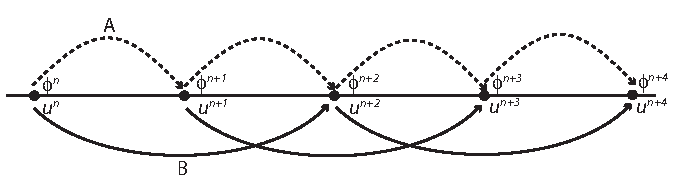
\includegraphics[width=12cm]{timestep}
\caption{Schematic depiction of the model time-step.  Note that in the
  code \emph{up} corresponds to $u^n$ and \emph{uc} corresponds to
  $u^{n+1}.$}
\label{fig:timestep}
\end{figure}

The model uses a hybrid time-stepping strategy.  At the top of the
timestep velocities are given at time level $n$ and $n+1$ and scalars
are given at time level $n.$ The scalars are then marched forward
using an Euler forward step to time-level $n+1.$ Velocities from
time-level $n$ are then taken forward using a leapfrog step to
time-level $n+2$ which concludes a single step.  On a timestep
tendencies are accumulated in a tendency array and then applied at the
end of the step.  An exception to this is the subgrid fluxes, which
involve what looks like a vertical diffusion operation.  The vertical
component of this operation is solved semi-implicitly which requires a
sparse matrix solve (a tri-diagnonal solver).  The new velocity is
then differenced with the old velocity to define an effective forward
tendency which is accumulated like the other forcings in the tendency
array.  Mathematically, if the time-level is indicated by a
superscript, then
\begin{equation}
\left( \frac{\partial \phi}{\partial t} \right)_{sgs} =
\frac{\tilde{\phi}^{n+1} - \phi^n}{\Delta t} \quad \text{where} \quad
\tilde{\phi}^{n+1} = \phi^n + \Delta t \frac{\partial}{\partial z}
\left(K^n \frac{\partial \tilde{\phi}^{n+1}} {\partial z} \right)
\end{equation}
and $K \equiv K_m/Pr$ is the eddy diffusivity.  Another exception is
the pressure gradient term which is solved so as to ensure that the
discretized version of
\begin{equation}
\frac{\partial}{\partial x_i} \left( \rho_0 \bar{u}_i\right) = 0
\end{equation}
is satisfied to machine precision.

The model employs a variable timestep, which is determined so as to
maintain the CFL with the range of 0.65 and 0.85.  If these bounds are
violated the timestep is adjusted back to the middle of the range.
This requires a recalculation of $u^{n+1}$ to make it consistent with
the new timestep, which we accomplish as follows:
\begin{equation} u^{n+1} = u^n +
  \frac{\Delta t} { \Delta \tilde{t} } ( \tilde{u}^{n+1} - u^n),
\end{equation} where $\tilde{u}^{n+1}$ and $\Delta \tilde{t}$ represent the
original values of $u^{n+1}$ and $\Delta t.$

\subsubsection{Computational Grid}

\begin{figure}
\centering \leavevmode 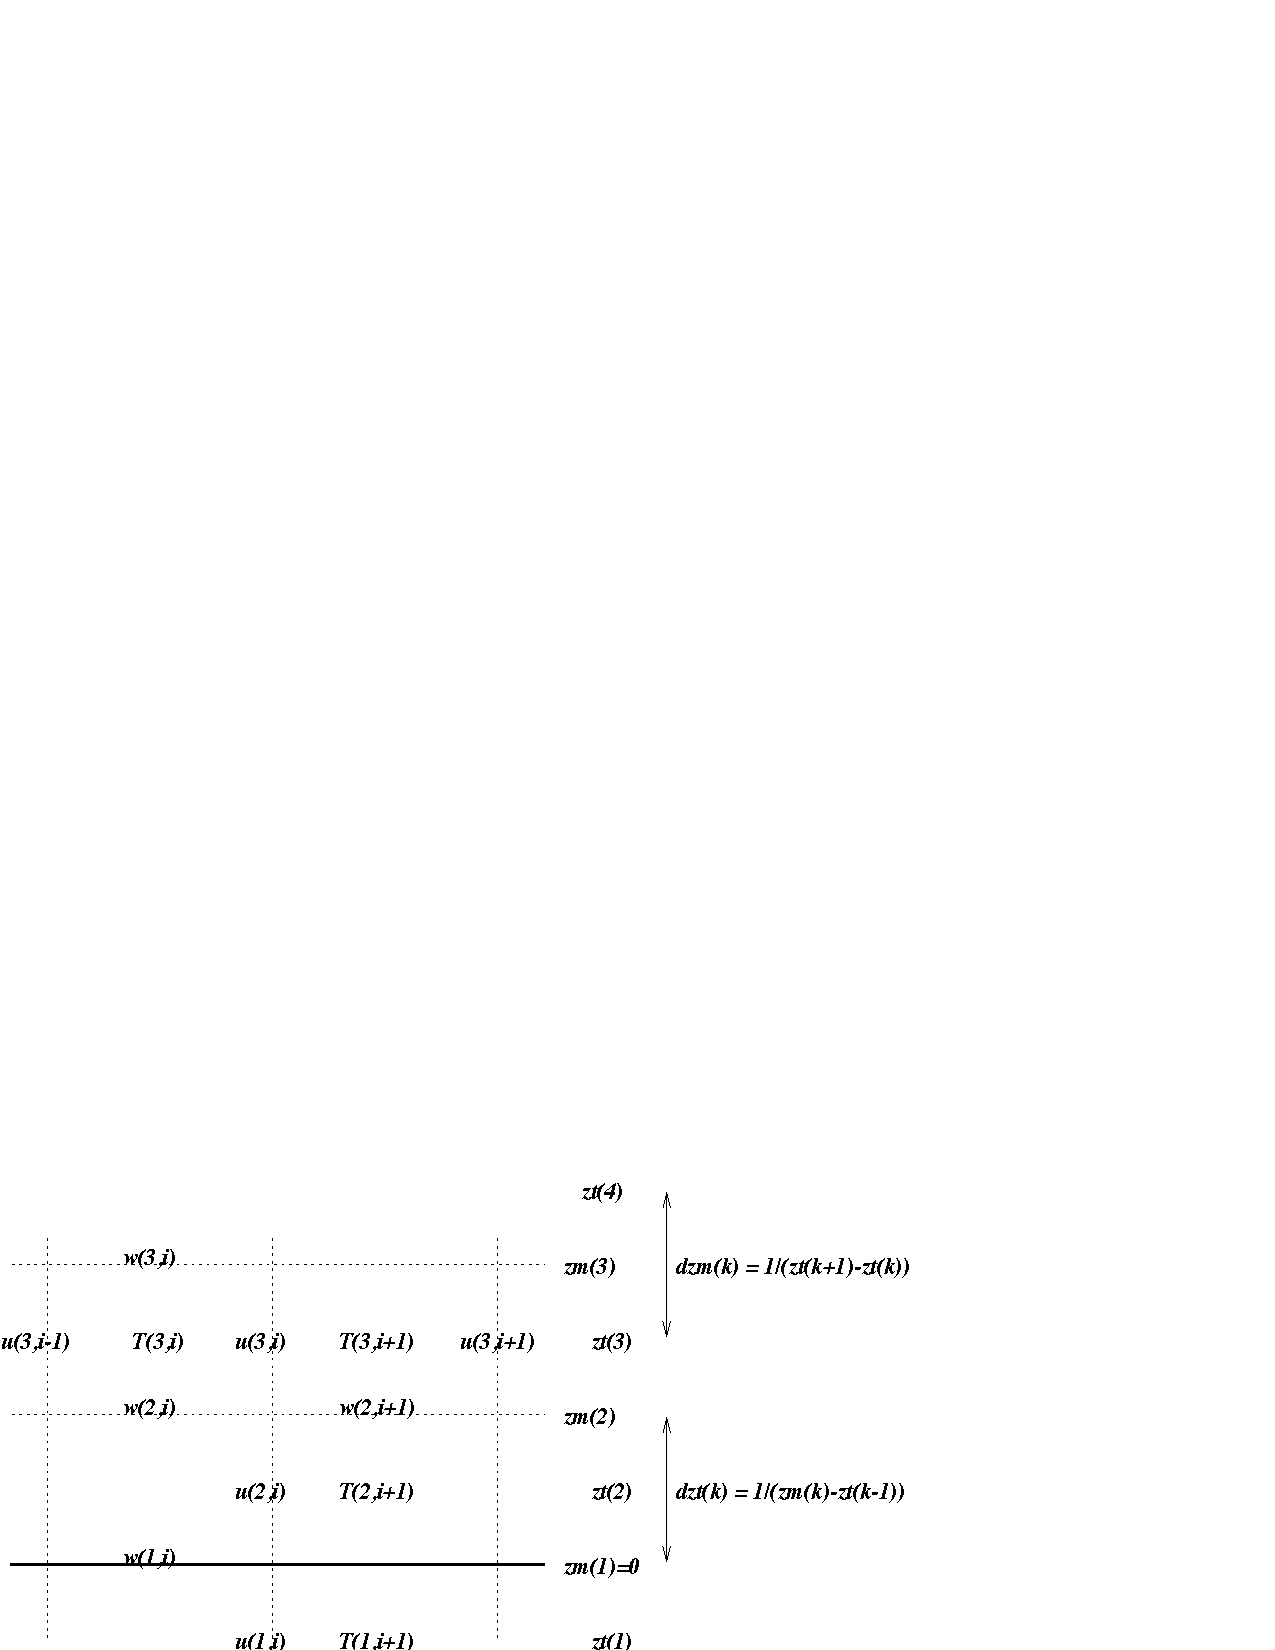
\includegraphics[width=12cm]{grid}
\caption{Schematic depiction of the model grid and where variables
locate on it.}
\label{fig:grid}
\end{figure}

The model uses the Arakawa-C grid, which means that $u(k,i,j)$ lies
$\frac{\Delta x}{2} $ meters to the right of $\theta_l(k,i,j)$ To
state this more generally, velocities are staggered half a grid point
up-grid (in the direction of the specific velocity component) of the
thermodynamic and pressure points.  Also note that the grid indexing
has the z dimension first.\footnote{Although given the way the model
is written, this is merely a social contract among the various
subroutines and thus could be changed.}  This $k,i,j$ indexing is
chosen in realization of the fact that many of the operations in the
model are done column-wise.  The grid configuration, and some height
variables that are commonly used in the code (i.e., \it zm, zt, dzm,
\rm and \it zt \rm) are illustrated in a schematic drawing in
Fig.~\ref{fig:grid}.

\subsubsection{Pressure Solver}

Pressure is solved by a fractional step method so as to ensure that
the velocities at the end of the timestep satisfy
(\ref{eq:continuity}) to machine accuracy.  The solver takes
advantage of the periodicity in the horizontal to use 2-D FFTs to
transform the Poisson-equation to a second order ODE in the
vertical. Schematically
\begin{equation}
\frac{\partial^2 \pi}{\partial x_i^2} \longrightarrow
(k^2+l^2)\frac{d^2\pi}{dz^2},
\end{equation}
where $k$ and $l$ denote the horizontal wave-numbers.  The resultant
ODE is then solved using a tri-diagnonal solver.

\subsection{Parallelization Strategy}

\subsubsection{Decomposition}
The parallelization is performed by decomposing the domain into
sub-domains consisting of strips in the $x$-$z$ plane.  This is a 1D
decomposition in that the parallelization is only along one of the
dimensions, $y.$  What results is $N_p$ $x$-$z$ slices consisting of
$N_y/N_p$ points in the $y$-direction.  Where $N_p$ denotes the number
of processors (strips) and $N_y$ is the total number of unique
$y$-points.  The way the memory is organized this has almost
no impact on the code but requires that the strips have at least two
unique $y$ points.  It also allows us to use domain-independent
indexing, so that $j \in \{1,\ldots,N_y/N_p+4\}$ where $j$ is the
$y-$index.  The addend of four represents the contribution from the
ghost points.  The width of the ghost-strips depends on the size of
the largest stencil used for a differencing computation in the code.
In our case the fourth order differences in the treatment of momentum
fluxes.  The effect of the
ghost-strips is to increase the number of grid-points.  The total
number of grid-points, $N_t$ is thus processor dependent.  The
overhead of the ghost-points can be measured by forming the ratio
$R(N_p) = N_t(N_p)/N_t(1).$  For the 1D decomposition with
ghost-strips two points deep:
\[ R(N_p) = 1 + 4\frac{N_p-1}{N_y+4} \]
For $N_p = N_y/2$ $\lim_{N_p\rightarrow\infty} R(N_p) = 3$.  Because
every computation need not be performed on a ghost point, the maximum
cost of the computation at the finest decomposition is some fraction
of this.  We have found that for sufficiently large domains the code
still scales well at its maximum possible decomposition.  That said
the best balance between efficiency and total time for execution is
usually found with $N_y/N_p$ around 8.

\subsubsection{Parallel I/O}
I/O is currently handled by each processor.  For binary history
writes MPI I/O is used to construct a single history file so as to
allow compatibility with sequential versions of the model. Otherwise,
statistical and analysis files are constructed for individual
sub-domains and then stitched together as necessary during the
post-processing.

\subsubsection{Communication} 
With the current 1-D parallelization strategy global communications
are only needed to implement boundary conditions, compute domain
integrals (such as means and co-variances), and calculate the FFTs.
The latter is the most significant issue.  Currently the FFTs are
first computed in the $x-$direction (along a strip), then the domain
is transposed into strips in the $y-$direction.  This makes use of the
fact that $N_y$ must equal $N_x$ in the current version of the code.
After the transpose the FFTs are computed in the $y$-direction and
then the vertical solver (tri-diagonal) solves the ODE (over $z$) in
the transpose space.  The inverse FFTs are then done in this transpose
space, then the inverse transpose is performed before computing the
inverse FFT along the strips in the $x$-direction.  This strategy only
requires two global communications per solve.

\subsubsection{Strategies for the Future} 
Because the 1-D decomposition limits the degree of parallelization
(the largest to date being a run on 256 processors) we are looking to
construct a version with a 2-D decomposition.  This would, in
principle, allow us to use $N_xN_y/4$ processors, i.e., more than 4
million with $N_x=N_y=4096.$ The normalized computational overhead
associated with the ghost strips would also be mitigated, with
\[R(N_p) = 1 + \frac{16(N_p-1) + 4(N_x+N_y)\sqrt{N_p}}{N_xN_y + 16} \]
For $N_x = N_y = 2\sqrt{N_p} \gg 1$ this ratio approaches 7, although
the communication overhead of such a large computation is more likely
to be the bottleneck.  In any case this appears to be a viable strategy
for taking advantage of machine architectures available in the
foreseeable future, but it would require more intensive communication,
perhaps at least four global communications per solve.

\section{The Code}

\subsection{Organization}

The distribution is spread among three directories: \emph{bin},
\emph{src}, \emph{misc}.  

The code itself resides in \emph{src} and is organized in F90 modules.
These are described in Table~\ref{tbl:modules}.  This directory also
contains two subdirectories \emph{seq} and \emph{mpi} where the
sequential or MPI modules are stored upon compilation.  In addition
rfft.F contains the Swartztrauber FFT routines which are called from
the util module, and omp\_interface.F90 contains and Open MP interface
which is under construction/consideration in support of finer grained
parallelization, but which is not used.  Lastly a Makefile here formed
by the master Makefile in \emph{bin} defines the specific
compilation/archive rules.  To add new modules requires modification
of this makefile.

\begin{table}
\begin{center}
\caption{Module F90 Files in \emph{src} directory} \label{tbl:modules}
\begin{tabular}[htb]{p{0.15\linewidth}p{0.85\linewidth}}
\hline \hline Module & Contains \\ \\  \hline
LES &  Main program which calls a timing
routine and the driver, as well as the driver subroutine and the
subroutine which defines and reads the model NAMELIST file. 
\\ advf &  Calculates the tendencies associated with scalar advection.
\\ advl &  Calculates the tendencies associated with momentum advection.
\\ defs &  Defines physical constants.
\\ forc &  Case specific forcings (radiation, subsidence, \emph{etc.})
\\ grid &  Definition of grid, allocation of memory and I/O management
\\ init &  Routines for processing input (either from
a file or the NAMELIST), definition of basic state, initialization of
fields, and definition of initial random perturbations.
\\ mcrp &  Bulk microphysical routines
\\ mpi\_interface & Definition of MPI parameters (use MPI) and MPI
routines for the domain decomposition
\\ mpi\_io & MPI I/O Routines
\\ prss &  Poisson solver, calculates the velocity tendencies
associated with pressure gradients, also implements time-filter for
leapfrog scheme and updates velocity.
\\ sgsm &  Subgrid scale solver.
\\ srfc &  Surface boundary condition  routines
\\stat &  Routines for calculating, accumulating and outputting model
statistics.  Statistical output is provided through the course of a
simulation and tends to be problem specific.
\\step &  Time stepper.  Also includes several routines for computing
tendencies due to physical processes (Coriolis force, buoyancy) or
boundary conditions (Rayleigh friction for sponge layer near lid).
Updating of scalars is done here. CFL computations and
timestep-regridding are also here.
\\thrm & Thermodynamic routines for calculating
quantities like temperature, and cloud water, given the thermodynamic
state of the model, i.e., $\theta_l,q_t,\rho_0,\pi_0,\Theta_0.$
\\util & A collection of basic utilities including
boundary conditions, FFT calls, explicit array operations such as
domain or slab averaging or covariances, the tri-diagonal solver, and
some NetCDF utilities.  Many of the routines in this module make
active MPI calls. \\ \hline
\end{tabular}
\end{center}
\end{table}

The \emph{bin} directory contains job control scripts and Makefiles.
The model is compiled from this directory (usually by typing make, or
make mpi, or make seq) and typically executed from here as well.  The
NAMELIST file defines any non-default input.

The \emph{misc} directory is a catchall for other useful things, for
instance alternative statistical or forcing routines are stored in
subdirectories.  Here code changes specific to past GCSS cases, or
idealized simulations such as free convection are stored.  To
implement them requires copying the appropriate code to the \emph{src}
directory and the appropriate NAMELIST to the \emph{bin} directory.
Codes used to construct initial soundings also appear hear.

\subsection{Compilation:}

To compile the model type ``make'' in the the \emph{bin} directory.
This will build the default version of the model using the default
architecture.  To compile the code on different machines
\emph{bin/Makefile} must be adjusted.  Currently there are settings to
compile on IBM, Macs with IBM/Motorola processors and the XLF
compiler, and Linux.  The code compiles and runs with G95 but our
experiences to date with this compiler suggest that it produces
executable which is a factor of two or more slower than commodity
compilers.

The model requires the NetCDF libraries to build, and where they
locate needs to be specified in \emph{bin.}  Our experiences with the
most aggressive optimization has been generally positive on the IBMs,
less so on the Mac.  Fine tuning the optimization can lead to
performance gains of 50\% or more, but aggressive optimisation (O3 or
greater on XLF compilers) should be checked.  For computations with
more than 128 points in a horizontal direction the code should be
promoted to double precision, if only to yield better defined global
integrals.  One such integral that ends up being important is the mean
buoyancy which must be subtracted from the local buoyancy so as to not
cause any mean accelerations.

\subsection{Specialized model configurations}

Perhaps the best way to learn how to configure the model for different
problems is to look at the configuration templates in the \emph{misc}
directories.  Here sub-directories (\emph{e.g.,} cumulus, gcss\_dycoms,
etc.,) contain substitute forcing, statistical and other modules, as
well as alternate NAMELIST files.  These are designed to run specific
past cases and produce output required by them.  Looking over how this
is done in the code could provide an example of how to set up your own
case, and statistical output.  Starting from a case that is close to
your desired objectives would naturally be the most straightforward
way to proceed.

\section{Running the model}

To run the model simply type the name of the executable, otherwise one
can submit it using a batch scheduler.  The latter is almost always
necessary in parallel programming environments.  Runs scripts used to
schedule the job using IBM Loadleveler or IBM Load Sharing protocols
are provided in the misc directory.

\subsection{The NAMELIST} 

Model execution can be controlled by NAMELIST parameters.  If a
NAMELIST parameter does not appear in the NAMELIST file for a
particular instance of the model execution, then the default for that
variable is assumed.  In Table \ref{tbl:namelist} we list the NAMELIST
variables, their default values, the module in which they locate, and
specialized behavior which can be obtained by specifying non-standard
NAMELIST values.

\begin{longtable}[htb]{p{0.1\linewidth}p{0.1\linewidth}p{0.1\linewidth}p{0.5\linewidth}}
\caption{NAMELIST variables and default values} \label{tbl:namelist}
\\ \hline \hline 
Variable & Module & Default Value & Comments \\ \hline \endhead
nxp & grid & 132 & total number of $x$ points ($N_y+4$) \\
nyp &  '' & 132 & total number of $y$ points ($N_y+4$) \\
nzp &  '' & 105 & total number of $z$ points \\
deltax & '' & 35.0 m & grid spacing in $x$-direction \\
deltay & '' & 35.0 m & grid spacing in $y$-direction \\
deltaz & '' & 37.5 m & grid spacing in $z$-direction \\
dzrat  & '' & 1.02   & grid stretching ration (default 2\% per
interval) \\
dzmax  & '' & 1200 m & height at which grid-stretching begins \\
dtlong & '' & 1.5 s  & maximum timestep \\
nfpt   & '' & 5      & number of levels in upper sponge layer \\
distim & '' & 300 s  & minimum relaxation time in sponge layer \\
th00   & '' & 288    & basic state potential temperature, $\Theta$ \\
igrdtyp & '' & 1 & Control parameter for selecting vertical grid \\
isgstyp & '' & 1 & Control parameter for selecting sgs model \\
iradtyp & '' & 1 & Control parameter for selecting radiation model \\
imcrtyp & '' & 1 & Control parameter for selecting microphysical model \\
naddsc  & '' & 0 &  Number of additional scalars \\
\\
CCN     & '' & 150 $\times 10^{6}$ & Cloud droplet mixing ratio \\
expnme  & '' & Default & Experiment name \\
filprf  & '' & test. & File prefix for use in constructing output files
\\ 
runtyp& ''   & INITIAL & Type of run ('INITIAL' or 'HISTORY') \\ \hline
ipsflg&  init  & 1   & control parameter for input sounding (0: pressure
in hPa; 1: height in meters with ps(1)= $p_{sfc}$) \\
itsflg&  ''  & 1   & control parameter for input sounding (0: ts =
$\theta;$ 1: $ts = \theta_l$) \\
us    &  ''  & n/a & input zonal wind souding (max nns=150 points) \\
vs    &  ''  & n/a & input meridional wind souding (max nns=150
points) \\
ts    &  ''  & n/a & input temperature souding (max nns=150 points) \\
rts   &  ''  & n/a & input humidity souding (max nns=150 points) \\
ps    &  ''  & n/a & input pressure sounding (max nns=150 points) \\
hs    &  ''  & n/a & vertical position (max nns=150 points) \\
iseed &  ''  & 0   &  random seed \\
zrand &  ''  & 200 m & height below which random perturbations are added \\
hfilin & ''  & test. & name of input history file for HISTORY starts
\\ \hline
timmax & step& 10800 s  &  final time of simulation \\ 
frqhis    & '' & 3600 s &  history write interval \\
frqanl    & '' & 3600 s &  analysis write interval  \\
outflg    & '' & True   &  output flag (true/false) \\
slcflg    & '' & False  &  write slice output (true/false) \\ 
istpfl    & '' & 1 &  print interval for timestep info \\
corflg    & '' & False   &  coriolis acceleration (true/false) \\
radfrq    & '' & 0   &  radiation update interval \\
strtim    & '' & 0   &  GMT of model time \\
cntlat    & '' & 31.5$^{\circ}$ N &  model central latitude \\  \hline
isfctyp   & srfc & 0  &  surface parameterization type (0: specified
fluxes; 1: specified surface layer gradients; 2: fixed lower boundary
of water \\
 ubmin     & '' & 0.20  &  minimum $u$ for $u_*$ computation \\
 zrough    & '' & -0.01 &  Momentum roughness height (if less than
 zero use Charnock relation)\\
 sst       & '' & 292 K &  Sea Surface Temperature \\
 dthcon    & '' &100 Wm$^{-2}$ &  Surface temperature gradient
 (itsflg=1) or surface heat flux (itsflg=0) \\
 drtcon    & '' &0   Wm$^{-2}$ &   Surface humidity (mixing ratio) gradient
 (itsflg=1) or surface latent heat flux (itsflg=0) \\ \hline
 csx       & sgsm &  0.23   &  Smagorinsky Coefficient \\
 prndtl    &  '' &  1/3    &  Prandtl Number (if less than zero no sgs for
 scalars) \\ \hline
savg\_intvl& stat & 1800 s    &  statistics averaging interval \\
ssam\_intvl&  '' &  30 s  &  statistics sampling interval
\\ \hline
\end{longtable}

The execution is controlled by a number of model parameters which are
given default specifications in the code. These specifications can be
modified in the NAMELIST file so as to allow multiple execution
without recompilation.  The full NAMELIST is defined in the LES.F90
subroutine and is described, along with default parameter values, in
Table \ref{tbl:namelist}.

\subsection{Output}

In addition to standard output, the model writes five types of files,
all of which are controlled by options in the NAMELIST file, and the
nature of the statistical routines in module \emph{stat}.

\paragraph{History files:} Fortran binary files which are given the name
\$(filprf)h.time where ``time'' is the time in seconds of the history
write and \$(filprf) is the string associated with \emph{filprf} in
the NAMELIST file.  History files contain the necessary data to
restart the model from a given time and integrate it forward.  If you
run the model for two hours and write a history file every hour, you
should be able to generate the data of the second hour identically by
restarting the model from the history file, \$(filprf)h.3600s written
at the end of the first hour and integrating forward for an hour.  In
addition three other types of history files are written
\$(filprf).iflg is written if the model is stopped due to a CFL
violation; \$(filprf).R at the first timestep; \$(filprf).h.rst is the
history state at the point when statistical averages are output (i.e.,
every savg\_intvl seconds this file is overwritten with the current
state).  Restarting from this file helps restart the model form the
latest data.

\paragraph{Analysis file:}  Space-time volumes that are useful for doing
data analysis on select three-dimensional fields are output
periodically.  In sequential runs this is a single file with the name
\$(filprf).nc, in parallel runs this consists of $N_p$ files, one for
each sub-domain with the name \$(filprf).\#\#\#\#.nc where \#\#\#\#
denotes the sub-domain number (beginning at 0). These data are
redundant with the history files, but less dense and in NetCDF, which
allows for more more frequent, output. 

\paragraph{Slice file:} Writes NetCDF output documenting the model
state for slices across the sub-domain. These are in $x-z,$ $y-z,$ and
$x-y.$   The naming convention is similar to that for analysis files,
but with the word ``slice'' included between the file prefix and its
suffix, i.e.,\$(filprf).slice.0012.nc for the 13th sub-domain.  These
files are most useful for writing output at very short temporal
intervals for making movies.

\paragraph{Profile statistics:}  This is a NetCDF file called
\$(filprf).ps.nc for a sequential run or \$(filprf).ps.\#\#\#\#.nc for
a parallel run.  It contains profile statistics averaged over the
averaging interval, with the number of samples determined by
savg\_intvl/ssam\_intvl (see Table \ref{tbl:namelist}).  The ability
of the model to calculate statistics on the fly can lead to more
economical output and more accurate statistics.  Our primary
motivation for doing this is, however, that in general it is very
important to use the same algorithm to calculate statistics (say
fluxes for instance) as is used by the model to timestep the field.
Given that, one might as well do the averaging during the course of a
run.  This method of averaging also makes it easier to generate finer
grained statistics.

\paragraph{Temporal Statistics:}  This is a netCDF file called
\$(filprf).ts.nc for a sequential run or \$(filprf).ts.\#\#\#\#.nc for
a parallel run.  It contains selected time-series statistics which can
be useful for getting a fine-grained view of the evolution of a
calculation.  Note that the parallel statistics are often computed
only over a sub-domain and deriving the appropriate domain averaged
quantity can be difficult.

\paragraph{Standard output:}  A number of fields are written to
standard output.  These include information about how the model is
configured and how long a timestep is taking.

\subsection{Post-processing:}

I perform almost all of my post-processing using NCL (the NCAR Command
Language).  This is a powerful data analysis, visualization,
file-handling scripting language that is free and distributed by NCAR
and handles NetCDF data intuitively.  In the \emph{misc/analysis}
directory are some NCL files I use to process data.  Similarly in
\emph{misc/synthesis} one should find the script reduce.ncl, which is
used to reduce statistical (ps and ts) files written over many
sub-domains to one file valid for the entire domain.

\paragraph{Other Useful Scripts:} \emph{misc/synthesis/rename.csh} 
is used to rename all the files produced by a run.  The file
\emph{misc/synthesis/reformat.ncl} was created to reformat the RICO
output to conform with the case specifications.  It provides an
example how to process the statistical data, particularly the
conditionally sampled data compiled over many
processors. \emph{misc/synthesis/call\_mss.csh} invokes
\emph{misc/scripts/mss.csh} to transfer files to the NCAR Mass storage
facility.  \emph{misc/scripts/resubmit.csh} resubmits jobs after
successful termination by changing the NAMELIST and calling the job
scheduler.  It was designed for the IBM SP systems.  In
\emph{misc/analysis} examples of plotting scripts are shown, these
include scripts for putting the model together to look at fields
spanning many processors (e.g., parallel.ncl).  As well as generic
scripts to plot files using ncl with command line arguments, i.e.,
plotfld.ncl, or a csh script plotfld.csh which invokes it.

\subsection{Debugging:}

My preferred way to debug the model is to track the evolution of the
model state using print statements.  I usually insert these between
subroutine calls to specific processes in the t\_step routine in
Module step so as to isolate problems.  When debugging it is useful to
have some idea of how physical variables relate to model variables,
which is the purpose of Table \ref{tbl:variables}.


\begin{longtable}[htb]{p{0.15\linewidth}p{0.15\linewidth}p{0.6\linewidth}}
\caption{Model variables} \label{tbl:variables}
\\ \hline \hline 
Array    & Dimensionality & Field \\ \hline \endhead
a\_up,a\_vp,a\_wp & 3D    & $u^n, \; v^n, \;w^n$ \\
a\_uc,a\_vc,a\_wc & ''    & $u^{n+1}, \;v^{n+1}, \;w^{n+1}$ \\
a\_ut,a\_vt,a\_wt & ''    & $\partial_t u, \; \partial_t v, 
\; \partial_t u$ \\  
a\_tp,a\_tt  & ''         & Liquid water potential temperature,
$\theta_l^{'\, n}, \;  \partial_t \theta_l$ \\ 
a\_rp,a\_rt  & ''         & Total water mixing ratio $r_t^n, \;
\partial_t r_t$ \\ 
a\_rpp,a\_rpt  & ''       & Rain mass mixing ratio $r_r^n, \;
\partial_t r_r$   (for level 3)\\  
a\_npp,a\_npt  & ''       & Rain number mixing ratio, $n_r^n, \;
\partial_t n_r$ (for level 3) \\  
a\_theta & '' & Potential temperature, $\theta$ (diagnosed from model state)
\\  
a\_rc,a\_rv  & ''         & Condensate and vapor mixing ratio $r_c, \;
r_v$ (note that $r_c$ can be either the cloud or total condensate
mixing ratio depending on when it is accessed) \\ 
a\_press, a\_pexnr & ''   & Pressure and Exner function, $p, \; \pi$
respectively  \\  
a\_scr1, a\_scr2 & '' & Three dimensional scratch arrays \\
a\_sclrp, a\_sclrt & 4D  & Additional scalars valid at time level $n$ and their tendency (4th dimension is naddsc and identifies which additional scalar). \\
a\_ustar, a\_tstar, a\_rstar & 2D & Surface scales, $u_*, \;
\theta_*, \; r_*$ respectively \\ 
uw\_sfc, vw\_sfc, ww\_sfc & '' & Surface momentum fluxes,
$\overline{u'w'}, \;\overline{v'w'}, \;\overline{w'w'} $
respectively. \\  
wt\_sfc, wq\_sfc & '' & Surface thermodynamic fluxes,
$\overline{w'\theta'}, \;\overline{w'r'} $
respectively. \\
precip & '' &  Precipitation flux \\
dn0    & 1D &  Basic state density, $\rho_0(z).$ \\
xt, yt, zt & '' & Position of thermodynamic points \\
xm, ym, zm & '' & position of momentum points \\
dzt        & '' & $1/(z_m(k) - z_m(k-1)$ \\
dzm        & '' & $1/(z_t(k+1) - z_t(k)$ \\
\hline
\end{longtable}

\section{Getting started}

In this section we show some basic profiles some of the basic cases.
By comparing your simulations with these you can get an idea if the
model is behaving as it should.  To help in these comparisons, sample
ps and ts files are provided for the smoke, rico and dry CBL (dcbl)
cases in the sub-directory \emph{doc/sample\_output}.

\paragraph{RICO:}  To run this case we copied all the 
\emph{misc/variants/gcss\_rico} source (F90) code into the source
directory and compiled the model.  The NAMELIST file was adapted (to
allow us to run in two stages) from the NAMELIST file also in the
gcss\_rico directory.  The run was performed in two stages on 64
processors (two virtual processors per real processor) using run.lsf
on the IBM power5 BlueVista Machine.  It took about 4.5 hours of real
time to compute 24 hours of simulated time.

\begin{figure}[htb]
\centering \leavevmode 
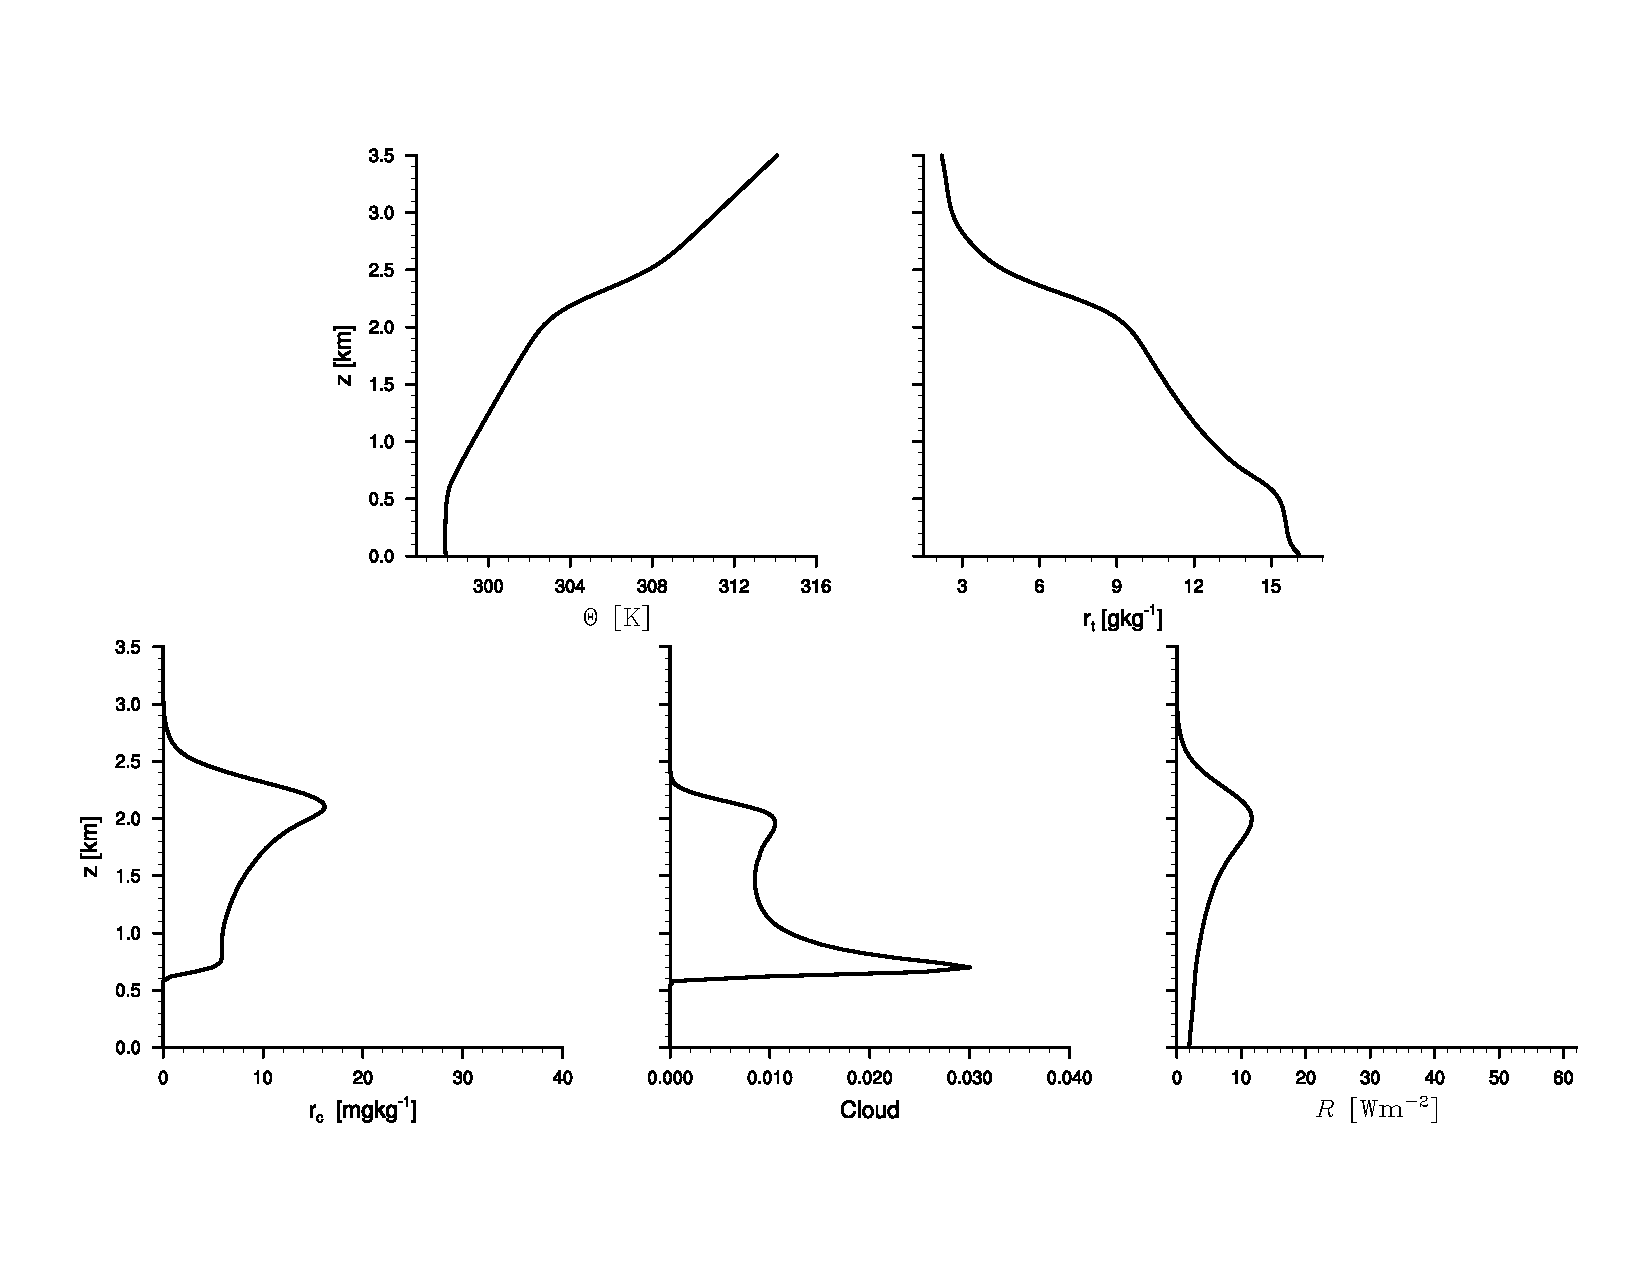
\includegraphics[width=10cm]{rico}
\caption{Thermodynamic profiles showing $\theta_l,$ $r_t,$ $r_c,$ core
cloud fraction and rain rate (in energetic units) averaged over the
last four hours of a 24 hour simulation.}
\label{fig:rico}
\end{figure}

The output was processed by first reducing the ts and ps files, then
reformatting them to the GCSS specifications, then plotting.  An
example of the thermodynamic state averaged over the last four hours
of the simulation is shown in Fig.~\ref{fig:rico}.  These results will
differ slightly from those submitted as part of the GCSS RICO
intercomparison because of slight changes used in the microphysics in
the present case, namely drop breakup and ventilation effects were
included.

\paragraph{Dry CBL:} To run this case we revert to the original or
default code by copying the \emph{misc/variants/original} source (F90)
code into the source directory and compile the model.  The NAMELIST
file was also taken from the \emph{original} directory.  The run was
performed using run.lsf on the IBM power5 BlueVista Machine.  It took
less than an hour to finish four hours of simulated time.

\begin{figure}[htb]
\centering \leavevmode 
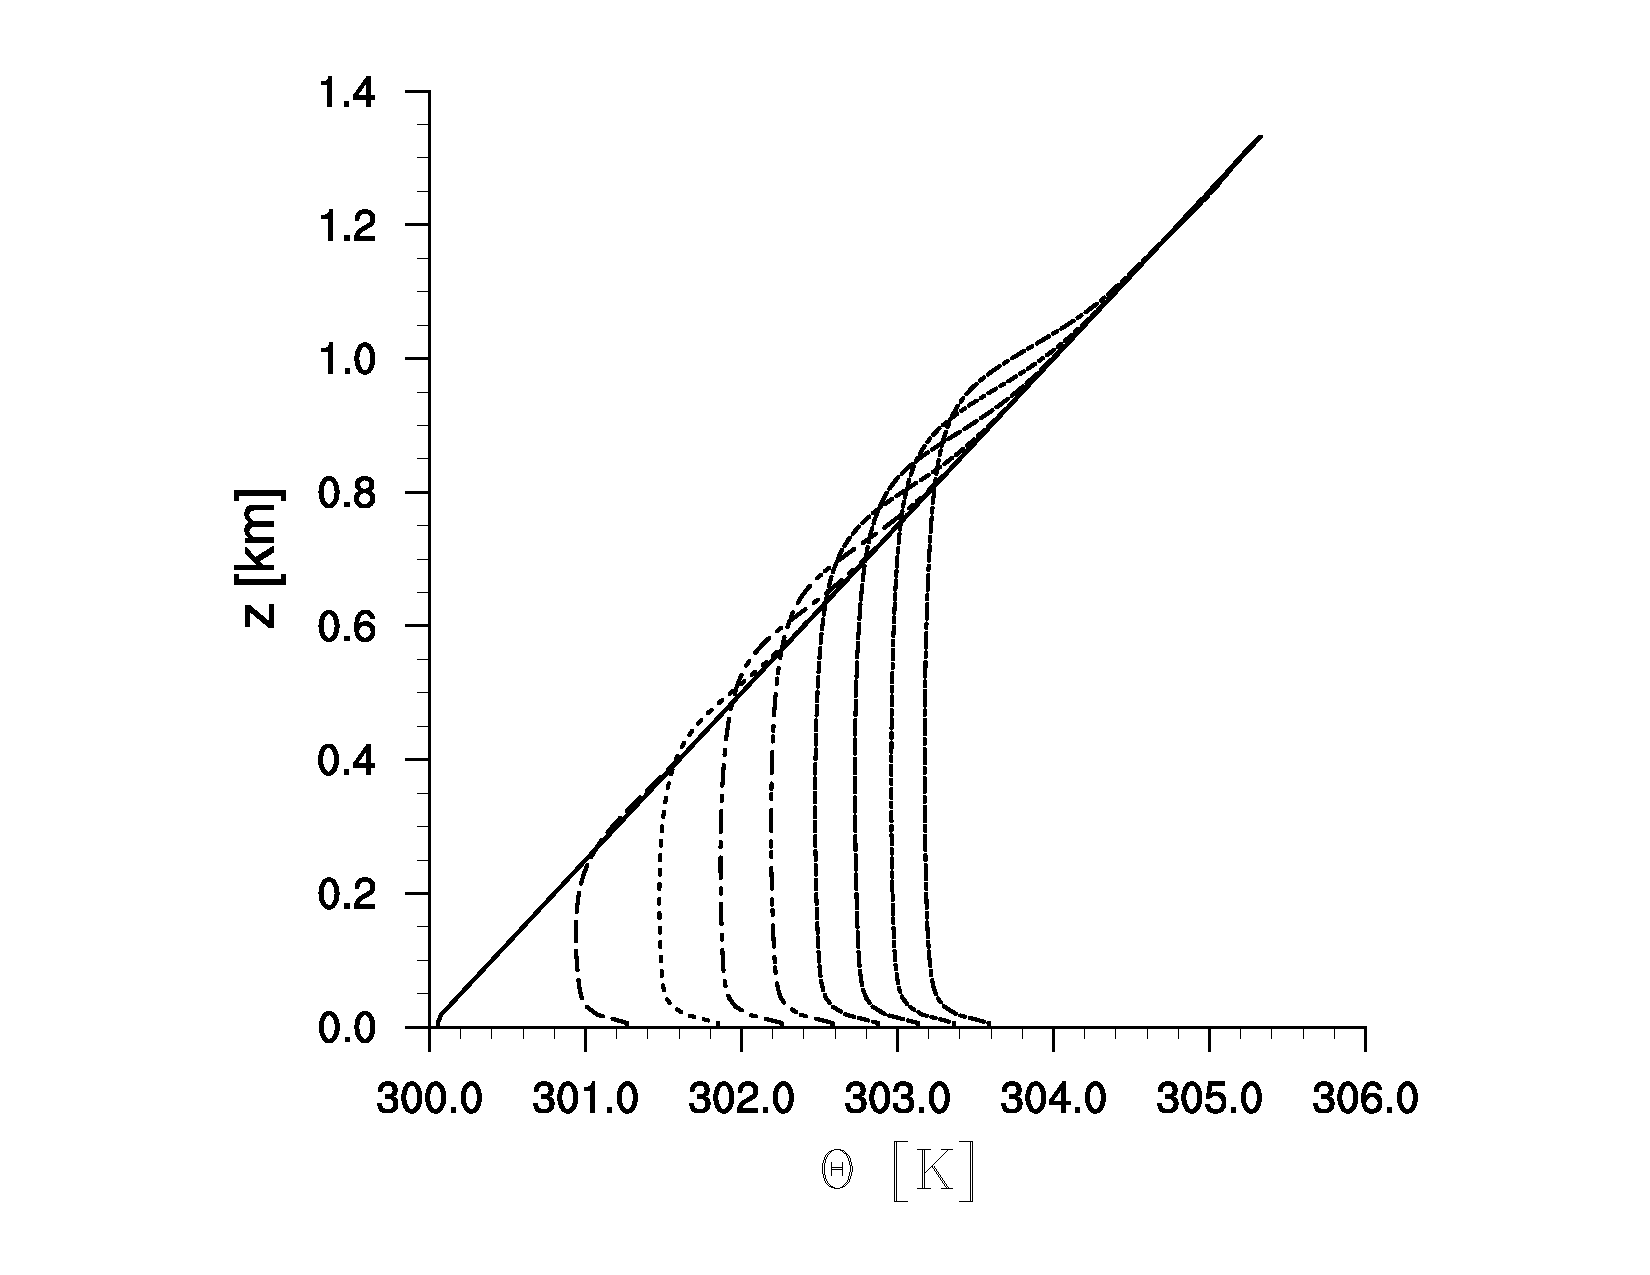
\includegraphics[width=8cm]{cbl}
\caption{Mean potential temperature profile for sample (default) dry
convective boundary layer simulation.  Profiles show profiles
averaged over 15 minutes plotted at 30 min intervals, with initial
state (actually state at the end of the first timestep) shown by solid
line.}
\label{fig:rico}
\end{figure}

The evolution of this run is shown in Figure \ref{fig:cbl} by the
profiles of $\theta$ at half hour intervals, where each profile is a
15 minute average.

\paragraph{Smoke:} 

\begin{figure}[htb]
\centering \leavevmode 
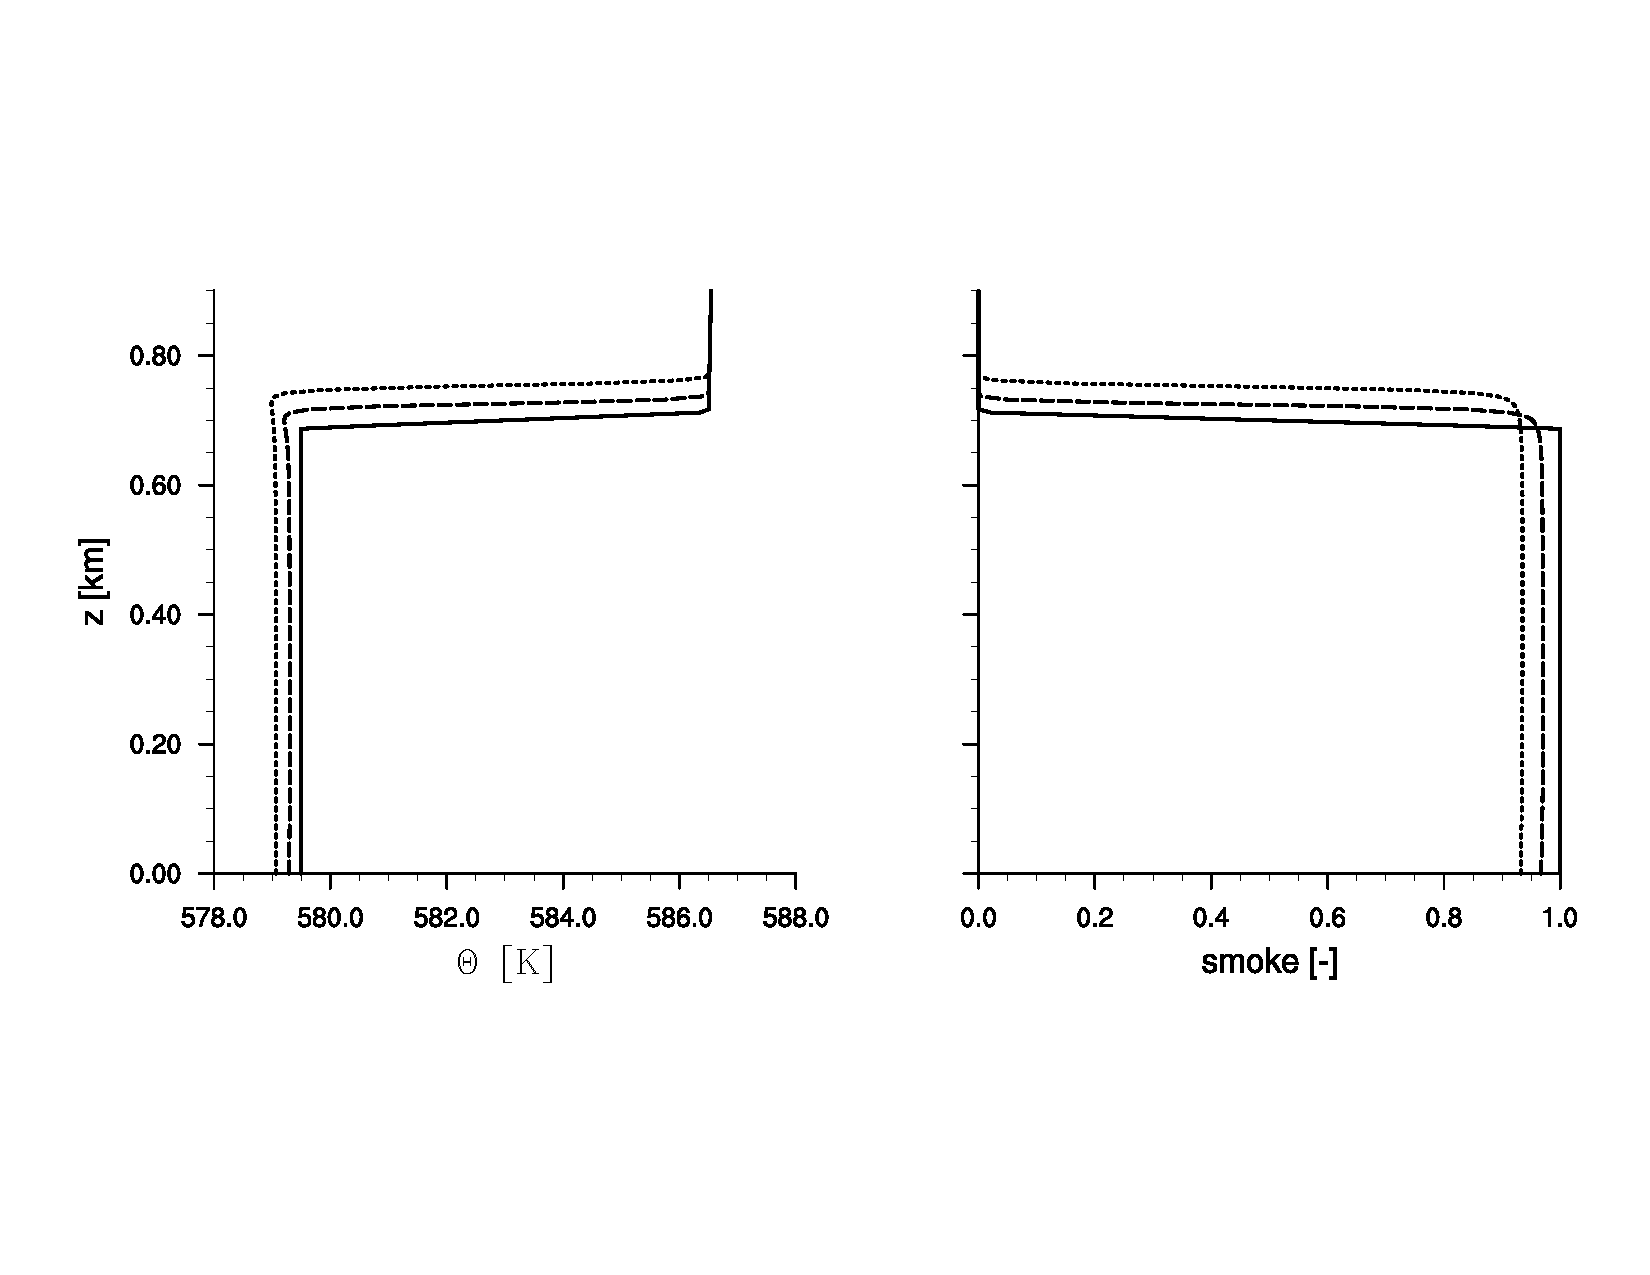
\includegraphics[width=12cm]{smoke}
\caption{Mean potential temperature profile for smoke cloud
simulation.  Shown oare profiles of $\theta $ and smoke concentration
averaged over 30 minutes plotted at 2 hr intervals, with initial state
(actually state at the end of the first timestep) shown by solid
line.}
\label{fig:smoke}
\end{figure}

Finally in Figure \ref{fig:smoke} we show the evolution of the smoke
cloud case.  For this plot we show the half hour averaged profiles for
the periods ending at 2 and 4 hrs.  The initial state is also shown by
the solid line.  What we see in the mean profiles is the expected
propagation of the smoke layer into the overlying fluid, accompanied
by the dilution of the smoke layer.  The slight instability at the top
of the smoke layer ($\theta$ decreasing with height) is the signature
of the radiative cooling active in this case.

\bibliography{/Users/bstevens/Documents/Latex/bibliography}

\end{document}












